\documentclass[11pt]{article}

\usepackage[margin=1in]{geometry}
\usepackage[T1]{fontenc}
\usepackage{lmodern}
\usepackage{microtype}
\usepackage{amsmath,amssymb,amsthm,mathtools}
\usepackage[dvipsnames]{xcolor}
\usepackage[most]{tcolorbox}
\usepackage{tikz}
\usepackage{enumitem}
\usepackage{tocloft}
\usepackage[hidelinks]{hyperref}

\definecolor{courseblue}{HTML}{1F4E79}
\definecolor{lightblue}{HTML}{EAF2F8}
\definecolor{lightgreen}{HTML}{EAF7EA}
\definecolor{lightpink}{HTML}{FCE8EF}
\definecolor{lightyellow}{HTML}{FFF8D6}
\definecolor{warningyellow}{HTML}{D6A000}
\definecolor{exercisebg}{HTML}{D6E6F5}
\definecolor{exerciseframe}{HTML}{1F4E79}
\definecolor{examplebg}{HTML}{F4FAFE}
\definecolor{exampleframe}{HTML}{85C1E9}
\definecolor{darkgray}{HTML}{333333}

\setlength{\parindent}{0pt}
\setlength{\parskip}{0.65em}
\setlist[itemize]{topsep=0.25em,itemsep=0.15em}
\renewcommand{\cftsecleader}{\cftdotfill{\cftdotsep}}
\renewcommand{\cftsubsecleader}{\cftdotfill{\cftdotsep}}

\theoremstyle{plain}
\newtheorem{theorem}{Theorem}[section]
\newtheorem{proposition}[theorem]{Proposition}
\newtheorem{lemma}[theorem]{Lemma}
\newtheorem{corollary}[theorem]{Corollary}
\theoremstyle{definition}
\newtheorem{definition}[theorem]{Definition}
\newtheorem{example}[theorem]{Example}
\newtheorem{exercise}[theorem]{Exercise}
\theoremstyle{remark}
\newtheorem*{remark}{Remark}
\newtheorem*{fact}{Fact}
\newtheorem*{warning}{Warning}

\tcolorboxenvironment{definition}{
  enhanced,
  colback=lightgreen,
  colframe=ForestGreen,
  boxrule=0.7pt,
  arc=2pt,
  left=6pt,
  right=6pt,
  top=5pt,
  bottom=5pt
}

\tcolorboxenvironment{warning}{
  enhanced,
  colback=lightyellow,
  colframe=warningyellow,
  boxrule=0.7pt,
  arc=2pt,
  left=6pt,
  right=6pt,
  top=5pt,
  bottom=5pt
}

\tcolorboxenvironment{exercise}{
  enhanced,
  colback=exercisebg,
  colframe=exerciseframe,
  boxrule=1pt,
  arc=2pt,
  left=6pt,
  right=6pt,
  top=5pt,
  bottom=5pt
}

\tcolorboxenvironment{example}{
  enhanced,
  colback=examplebg,
  colframe=exampleframe,
  boxrule=0.7pt,
  arc=2pt,
  left=6pt,
  right=6pt,
  top=5pt,
  bottom=5pt
}

\numberwithin{equation}{section}

\newcommand{\be}{\begin{eqnarray}}
\newcommand{\ee}{\end{eqnarray}}
\newcommand{\C}{\mathbb{C}}
\newcommand{\R}{\mathbb{R}}
\newcommand{\N}{\mathbb{N}}

\DeclareMathOperator{\Hol}{\mathcal{H}\mathrm{ol}}
\DeclareMathOperator{\Real}{Re}
\DeclareMathOperator{\Imag}{Im}
\newcommand{\A}{\mathcal{A}}
\newcommand{\CT}{\C[[T]]}
\newcommand{\CLT}{\C((T))}
\tcbset{breakable}
\begin{document}

\begin{center}
  \colorbox{lightblue}{%
    \begin{minipage}{0.94\textwidth}
      \vspace{0.55em}
      \begin{tabular*}{\textwidth}{@{\extracolsep{\fill}}lr}
        {\color{courseblue}\bfseries\LARGE Lecture 9} &
        {\color{courseblue}\bfseries\LARGE MATH 411}\\[0.35em]
        \textbf{Fall 2026} & \textbf{Date: Sep 23, 2026}\\
        & \textbf{Instructor: Manish Patnaik}
      \end{tabular*}
      \vspace{0.45em}
    \end{minipage}}
\end{center}

\setcounter{tocdepth}{1}
\tableofcontents
\vspace{0.45em}

% Handwritten page 1.
\section{Recollections}
To a formal power series $f(T)=\sum a_nT^n\in\CT$ we have assigned an
extended nonnegative number $r\in[0,\infty]$, the \emph{radius of
convergence}, such that
\be
 f(z)=\sum a_nz^n
\ee
converges absolutely at every point of $D(0,r)$, converges uniformly on every
closed disc $\overline{D(0,s)}$ with $s<r$, and diverges for $|z|>r$.
Hadamard's criterion computes it from the coefficients:
\be
 \limsup_{n}|a_n|^{1/n}=\frac1r.
\ee

\begin{example}
Consider $\sum n!\,z^n$. By Stirling, $n!=n^ne^{-n}u_n$ with
$\lim_{n\to\infty}u_n^{1/n}=1$, so
\be
 \limsup_{n}|n!|^{1/n}=\limsup_{n}\;n\,e^{-1}u_n^{1/n}=\infty.
\ee
Hence the radius of convergence is $\dfrac1\infty=0$: the series converges
only at $z=0$.
\end{example}

\section{The formal derivative has the same radius of convergence}
Suppose $f(T)=\sum a_nT^n$ has radius of convergence $r$. Its
\emph{formal derivative} is
\be
 f'(T)=\sum_{n\geq1}n\,a_nT^{n-1}.
\ee

% Handwritten page 2.
\begin{proposition}
\label{prop:roc-derivative}
The formal derivative $\sum_{n\geq1}n\,a_nz^{n-1}$ has radius of convergence
$r$ as well.
\end{proposition}

\begin{proof}
First consider the formal series $T f'(T)=\sum_{n\geq1}n\,a_nT^n$. Since
$n^{1/n}\to1$, Hadamard's criterion gives
\be
 \limsup_{n\to\infty}n^{1/n}|a_n|^{1/n}
 =\limsup_{n\to\infty}|a_n|^{1/n}
 =\frac1r,
\ee
where
\be
 n^{1/n}=e^{\frac1n\log n}\longrightarrow e^0=1.
\ee
Thus $T f'(T)$ has radius $r$. Removing the initial zero coefficient and
shifting the powers down by one does not change a power series's radius of
convergence, so $f'(T)$ also has radius $r$.
\end{proof}

\section{A convergent power series is \texorpdfstring{$\C$}{C}-differentiable}
Let $f(z)=\sum a_nz^n$ be a power series with radius of convergence $r$ and regard it as a function on $D(0,r)$. \emph{Question.} What is the relation between $f'(z)$ --- the derivative we
discussed earlier --- and \be \sum_{n\geq1}n\,a_nz^{n-1} ? \ee

To address this, we must first ask what kind of function $f(z)$ is. On every
closed disc $\overline{D(0,s)}$ with $s<r$, it is a uniform limit of
$\C$-differentiable functions, namely the partial sums
\be
 S_k=\sum_{n=0}^{k}a_nz^n\longrightarrow f.
\ee

\begin{warning}
A uniform limit of differentiable functions need not be differentiable in
the real-variable setting. For example, the functions
\be
 f_n(x)=\sqrt{x^2+\tfrac1n}\qquad(x\in\R)
\ee
are differentiable (indeed smooth) on $\R$, and they converge uniformly to
$|x|$, since
\be
 0\leq\sqrt{x^2+\tfrac1n}-|x|
 =\frac{1/n}{\sqrt{x^2+\frac1n}+|x|}
 \leq\frac1{\sqrt n}.
\ee
Yet the limit $|x|$ is not differentiable at $x=0$. (If you have seen it before, then the 
Weierstrass approximation theorem states that every continuous function on $[a,b]$ --- even a
nowhere-differentiable one --- is a uniform limit of polynomials.)
\end{warning}

\begin{theorem}
\label{thm:ps-diff}
The function $f(z)=\sum a_nz^n$ is $\C$-differentiable on its region of
convergence $D(0,r)$.
\end{theorem}

% Handwritten page 3.
\begin{proof}
Fix $z\in D(0,r)$ and choose $\rho$ with $|z|<\rho<r$. For
$0<|h|<\rho-|z|$, the binomial theorem gives
\be
 (z+h)^n-z^n-nz^{n-1}h=h^2P_n(z,h),
 \qquad
 P_n(z,h):=\sum_{k=2}^{n}\binom nk z^{n-k}h^{k-2}.
\ee
For $2\leq k\leq n$, we have
$\binom nk\leq\binom n2\binom{n-2}{k-2}$. Hence
\begin{align*}
 |P_n(z,h)|
 &\leq \binom n2
   \sum_{k=2}^{n}\binom{n-2}{k-2}|z|^{n-k}|h|^{k-2}\\
 &=\binom n2(|z|+|h|)^{n-2}
 \leq\binom n2\rho^{n-2}.
\end{align*}
The last inequality is where the choice of $\rho$ enters: for the admissible
increments $h$, the points $z+h$ fill the disc $D(z,\rho-|z|)$, and every such
$h$ satisfies $|z|+|h|<\rho<r$.

\begin{center}
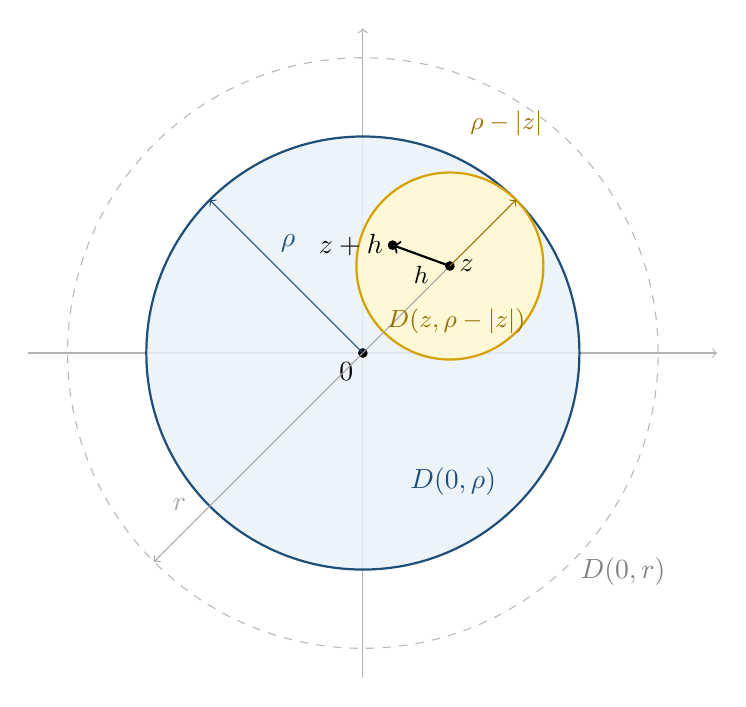
\begin{tikzpicture}[scale=1.25]
  % axes
  \draw[->,gray!60] (-3.4,0) -- (3.6,0);
  \draw[->,gray!60] (0,-3.3) -- (0,3.3);
  % region of convergence and the intermediate disc
  \draw[gray!55,dashed] (0,0) circle (3);
  \fill[lightblue,opacity=0.85] (0,0) circle (2.2);
  \draw[courseblue,thick] (0,0) circle (2.2);
  % admissible points z+h
  \coordinate (z) at (45:1.25);
  \fill[lightyellow] (z) circle (0.95);
  \draw[warningyellow,thick] (z) circle (0.95);
  % points
  \fill (0,0) circle (1.4pt) node[below left]{$0$};
  \draw[gray!70] (0,0) -- (z);
  \fill (z) circle (1.4pt) node[right]{$z$};
  \path (z) ++(160:0.62) coordinate (zh);
  \draw[->,thick] (z) -- (zh) node[midway,below,font=\small]{$h$};
  \fill (zh) circle (1.4pt) node[left]{$z+h$};
  % radii
  \draw[gray!70,->] (0,0) -- (225:3) node[pos=0.8,above left]{$r$};
  \draw[courseblue,->] (0,0) -- (135:2.2) node[pos=0.6,above right]{$\rho$};
  \draw[warningyellow!70!black,->] (z) -- ++(45:0.95);
  \node[warningyellow!70!black,font=\small] at (58:2.75) {$\rho-|z|$};
  % labels
  \node[gray] at (-40:3.45) {$D(0,r)$};
  \node[courseblue] at (-55:1.6) {$D(0,\rho)$};
  \node[warningyellow!70!black,font=\small] at (0.95,0.32) {$D(z,\rho-|z|)$};
\end{tikzpicture}
\end{center}

% Handwritten page 4.
By Proposition~\ref{prop:roc-derivative}, applied twice, the series
\be
 M_\rho:=\sum_{n=2}^{\infty}\binom n2|a_n|\rho^{n-2}
\ee
converges. Also, the series
\be
 \alpha:=\sum_{n=1}^{\infty}n\,a_nz^{n-1}
\ee
converges. Therefore
\begin{align*}
 \left|\frac{f(z+h)-f(z)}{h}-\alpha\right|
 &\leq |h|\sum_{n=2}^{\infty}|a_n|\,|P_n(z,h)|\\
 &\leq |h|M_\rho\longrightarrow0
 \qquad\text{as }h\to0.
\end{align*}
Thus $f$ is $\C$-differentiable at $z$, with $f'(z)=\alpha$.
\end{proof}

\begin{remark}
So $f(z)=\sum a_nz^n$ is $\C$-differentiable on $D(0,r)$ and
\be
 f'(z)=\alpha=\sum_{n=1}^{\infty}n\,a_nz^{n-1},
\ee
i.e.\ a power series may be differentiated term by term inside its disc of
convergence.
\end{remark}

% Handwritten page 5.
In fact the same analysis applies to
$f'(z)=\sum_{n=1}^{\infty}n\,a_nz^{n-1}$ to show that it too is
differentiable, with derivative
\be
 \sum_{n=2}^{\infty}n(n-1)a_nz^{n-2},
\ee
and so on: $f$ is infinitely $\C$-differentiable on $D(0,r)$.

\section{Analytic functions}

\begin{definition}[Analytic]
Let $U\subseteq\C$ be an open set. A function $f\colon U\to\C$ is said to be
\emph{analytic at $z_0\in U$} if there exist $\rho>0$ and a power series
$\sum a_nT^n$, with radius of convergence at least $\rho$, such that
$D(z_0,\rho)\subseteq U$ and
\be
 f(z)=\sum a_n(z-z_0)^n\qquad\text{for all }|z-z_0|<\rho,
\ee
i.e.\ for all $z\in D(z_0,\rho)$. If $f$ is analytic at each point $z_0\in U$,
we say $f$ is \emph{analytic on $U$}.
\end{definition}

\begin{theorem}
\label{thm:ps-analytic}
Let $f(T)=\sum a_nT^n$ have radius of convergence $r$. Then the function
$f(z)=\sum a_nz^n$ that it defines is analytic on all of $D(0,r)$.
\end{theorem}

% Handwritten page 6.
\begin{proof}
Pick $z_0\in D(0,r)$ and choose $s>0$ such that $|z_0|+s<r$. We seek a
power series expansion around $z_0$ of the form
\be
 f(z)=\sum b_k(z-z_0)^k\qquad\text{for }z\in D(z_0,s),
\ee
whose radius of convergence is at least $s$. For such $z$,
\be
 z=z_0+(z-z_0),\qquad |z|\le|z_0|+|z-z_0|<r,
\ee
so $z\in D(0,r)$ and $f(z)$ makes sense. Now expand
\be
 z^n=\sum_{k=0}^{n}\binom nk z_0^{\,n-k}(z-z_0)^k,
\ee
so that
\be
 f(z)=\sum_n a_nz^n
 =\sum_n a_n\left(\sum_{k=0}^{n}\binom nk z_0^{\,n-k}(z-z_0)^k\right).
\ee
For each $k\geq0$, the series
\be
 b_k:=\sum_{n=k}^{\infty}\binom nk z_0^{\,n-k}a_n
\ee
converges absolutely: up to the factor $1/k!$, it is the formally
differentiated series of order $k$ evaluated at $z_0$, and that series still
has radius $r$ by Proposition~\ref{prop:roc-derivative}.
The resulting double series is absolutely convergent because
\begin{align*}
 &\sum_{n=0}^{\infty}\sum_{k=0}^{n}
 |a_n|\binom nk|z_0|^{n-k}|z-z_0|^k\\
 &\hspace{4em}=
 \sum_{n=0}^{\infty}|a_n|\bigl(|z_0|+|z-z_0|\bigr)^n<\infty.
\end{align*}
We may therefore rearrange the terms and obtain
\be
 f(z)=\sum_{k=0}^{\infty}b_k(z-z_0)^k,
\ee
and $\sum b_kT^k$ converges absolutely for every $|T|<s$. It therefore has
radius of convergence at least $s>0$, proving that $f$ is analytic at $z_0$.
\end{proof}

% Handwritten page 7.
\begin{example}
Let
\be
 f(z)=\frac{z^2}{z+2}.
\ee
\textbf{Near $0$:}
\be
 \frac{z^2}{z+2}=z^2\left(\frac1{\frac z2+1}\right)\cdot\frac12
 =\frac12z^2\left(1-\frac z2+\frac{z^2}4-\frac{z^3}8+\cdots\right),
\ee
which has radius of convergence $2$ --- the distance from $0$ to the pole at
$z=-2$.

\textbf{Near $z=1$:} writing $z=1+(z-1)$,
\be
 f(z)=\frac{z^2}{z+2}=\frac{\bigl(1+(z-1)\bigr)^2}{1+(z-1)+2}
 =\frac13+\frac59(z-1)+\cdots,
\ee
and this expansion has radius of convergence $3$, again the distance from
the centre $1$ to the pole at $-2$.
\end{example}

\noindent
\begin{minipage}[c]{0.42\textwidth}
\centering
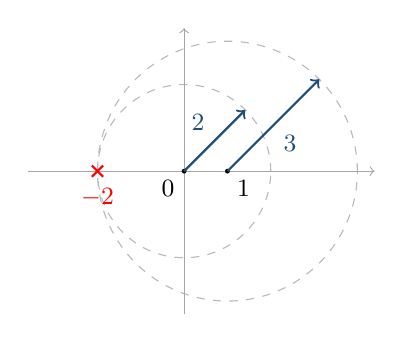
\begin{tikzpicture}[scale=0.55,every node/.style={font=\small}]
  \draw[gray!55,dashed] (0,0) circle (2);
  \draw[gray!55,dashed] (1,0) circle (3);
  \draw[->,gray!70] (-3.6,0) -- (4.4,0);
  \draw[->,gray!70] (0,-3.3) -- (0,3.3);
  \fill (0,0) circle (1.6pt) node[below left]{$0$};
  \fill (1,0) circle (1.6pt) node[below right]{$1$};
  \draw[red,thick] (-2.13,-0.13) -- (-1.87,0.13);
  \draw[red,thick] (-2.13,0.13) -- (-1.87,-0.13);
  \node[red,below] at (-2,-0.18) {$-2$};
  \draw[courseblue,thick,->] (0,0) -- (1.41,1.41) node[midway,above left]{$2$};
  \draw[courseblue,thick,->] (1,0) -- (3.12,2.12) node[midway,below right]{$3$};
\end{tikzpicture}
\end{minipage}\hfill
\begin{minipage}[c]{0.55\textwidth}
\begin{remark}
In both cases the radius of convergence is exactly the distance from the
centre of expansion to the nearest point where $f$ fails to be defined. This
is not an accident, and we will return to it.
\end{remark}
\end{minipage}

\begin{exercise}
Expand $f(z)=\dfrac{z^2}{z+2}$ around $z_0=-1$ and check that the radius of
convergence you obtain from Hadamard's criterion equals $|-1-(-2)|=1$.
\end{exercise}

\end{document}
